\documentclass[12pt, a4paper]{article}

\usepackage[utf8]{inputenc}

\usepackage{ifxetex,ifluatex}
\usepackage{etoolbox}
\usepackage[svgnames]{xcolor}

\usepackage{tikz}

\usepackage{framed}

% conditional for xetex or luatex
\newif\ifxetexorluatex
\ifxetex
  \xetexorluatextrue
\else
  \ifluatex
    \xetexorluatextrue
  \else
    \xetexorluatexfalse
  \fi
\fi
%
\ifxetexorluatex%
  \usepackage{fontspec}
  \usepackage{libertine} % or use \setmainfont to choose any font on your system
  \newfontfamily\quotefont[Ligatures=TeX]{Linux Libertine O} % selects Libertine as the quote font
\else
  \usepackage[utf8]{inputenc}
  \usepackage[T1]{fontenc}
  \usepackage{libertine} % or any other font package
  \newcommand*\quotefont{\fontfamily{LinuxLibertineT-LF}} % selects Libertine as the quote font
\fi

\newcommand*\quotesize{60} % if quote size changes, need a way to make shifts relative
% Make commands for the quotes
\newcommand*{\openquote}
   {\tikz[remember picture,overlay,xshift=-4ex,yshift=-2.5ex]
   \node (OQ) {\quotefont\fontsize{\quotesize}{\quotesize}\selectfont``};\kern0pt}

\newcommand*{\closequote}[1]
  {\tikz[remember picture,overlay,xshift=4ex,yshift={#1}]
   \node (CQ) {\quotefont\fontsize{\quotesize}{\quotesize}\selectfont''};}

% select a colour for the shading
\colorlet{shadecolor}{Azure}

\newcommand*\shadedauthorformat{\emph} % define format for the author argument

% Now a command to allow left, right and centre alignment of the author
\newcommand*\authoralign[1]{
 	\def\authorfill{\hfill}\def\quotefill{}
}
% wrap everything in its own environment which takes one argument (author) and one optional argument
% specifying the alignment [l, r or c]
%
\newenvironment{shadequote}[2][l]%
{\authoralign{#1}
\ifblank{#2}
   {\def\shadequoteauthor{}\def\yshift{-2ex}\def\quotefill{\hfill}}
   {\def\shadequoteauthor{\par\authorfill\shadedauthorformat{#2}}\def\yshift{2ex}}
\begin{snugshade}\begin{quote}\openquote}
{\shadequoteauthor\quotefill\closequote{\yshift}\end{quote}\end{snugshade}}


%----------------------------------------%


% Package to use images
\usepackage{graphicx}
\graphicspath{{img/}}

\usepackage[utf8]{inputenc}

% Package to import PDF documents (for page2)
\usepackage[final]{pdfpages}

% Package to use tables
\usepackage{tabularx}



% No indent at pargagraph
\setlength{\parindent}{0pt} 

% To the code snipping
\usepackage{listings}
\lstset{
    tabsize=2,
    numbers=left,
  	stepnumber=1,    
  	firstnumber=1,
  	numberfirstline=true,
  	xleftmargin=6mm
}

% Inline code test
\newcommand{\code}[1]{{\small \texttt{#1}}}


\begin{document}

% Front page
\begin{titlepage}

\Large Automasjon 2016 \\

\vspace{3cm}

\begin{center}
\Huge The analysis of C\# to F\# \vspace{10mm}\\
\large Jostein Andreassen, Michael Blomli and Mikkel Eltervåg \vspace{3mm}\\
Automation \vspace{5mm}\\
12. May 2015
\end{center}

\vspace{5cm}

\begin{figure}[!h]
  \centering
  \begin{minipage}[b]{0.3\textwidth}
    \includegraphics[width=\textwidth]{fsharp128}
  \end{minipage}
  \hfill
  \begin{minipage}[b]{0.3\textwidth}
    \includegraphics[width=\textwidth]{serit_logo}
  \end{minipage}
  \hfill
  \begin{minipage}[b]{0.3\textwidth}
    \includegraphics[width=\textwidth]{LogoEngelsk}
  \end{minipage}
\end{figure}


\end{titlepage}

\newpage

%Page 2 from PDF
\includepdf[pages=-]{page2.pdf}

\newpage
\section*{Summary}
This report is written by 3 students from the final year in the Automation class at “UiT: University of Tromsø - Arctic university of Norway”.\\

The assignment is given by a company named Serit - IT Partner from Tromsø. They wanted us to find out the benefits, flaws and our experience from learning a new programming language called F\#. Today Serit mostly uses the famous programming language C\# which is widely used around the world today. The time spent writing code, debugging and stability in these languages is very valuable.

\newpage
\section*{Preface}
This thesis is written by graduates from the automation program at the department of engineering  at UiT: University of Tromsø - Norway's Arctic university. This thesis will be used by Serit to help them decide if they are going to incorporate the programming language F\# or not.\\

We chose this assignment because everyone in our group enjoys programming, it had some database management and set up, and because it looked like an interesting project overall. Since we already had some experience in C\#, we thought it would be fun to find the “pros and cons” of this relatively new programming language.\\

We have written the thesis in LaTeX which is a word processor and a document markup language. When we were working on the raw text we used Google documents so that we all could work together simultaneously on writing and editing the text for the thesis. On the main assignment we used Visual Studio (with C\# and F\# tools), Atlassian Sourcetree and Github to write and manage our code, and SQL Server Management Studio to handle the database. By using both C\# and database we covered a wide area of our education from the previous semester. We have learnt a lot and have had the privilege of testing out the new attractive programming language F\# that may just be the future.\\ 

We want to give out a special thanks to Serit for all the great support and advice given, on all the regular follow up meetings we had and by email. We also want to give a big thanks to our mentor Puneet Sharma for his great support and contribution to the assignment.

\newpage
\tableofcontents

\newpage
\section{Introduction}
\subsection{Background}
One of the biggest problems in modern application development is the rapidly growing complexity of all major software systems. This complexity makes it almost impossible to ensure the quality and accuracy of the code. It also becomes harder and harder to make changes to existing code without introducing new errors. All these difficulties multiply when you also want utilize modern computers with many CPU (central processing unit) cores for increased performance.\\

The imperative object-oriented programming paradigm has been dominant in software development for over 20 years. In the imperative paradigm the state variables will be handled explicitly, which can quickly give too much complexity. The functional programming paradigm has been known since the 1930’s, but has not been popular with professional developers because of the slightly lower (single core) performance and greater resource use. Today these obstacles are long gone, and functional programming is experiencing a new renaissance due to significantly better control over complexity and parallelism.\\

We've received an assignment from Serit to translate parts of an existing project from C\# code to F\# code. C\# is meant to be simple, modern, flexible and object oriented programming language. It  is developed and maintained by Microsoft and is inspired by previous popular object-oriented languages like C++ and Java. F\# is a hybrid language that supports both the familiar object-oriented method and functional programming. F\# is also developed by Microsoft, and like C\# also has access to Microsoft’s .NET framework. Serit wants us to find out the benefits of  switching from development in the programming language C\# development to F\#.\\

\newpage
\subsection{Problem for discussion}
C\# and F\# works in different ways, they both have benefits and drawbacks. The main question is if it is worth it for a company to change their main programming language. We have to look at what the company wants to achieve by making the change, and that boils down to making quality programs for a low price. \\

A modern IT company uses a lot of time developing, changing and fixing code. If we can use a programming language that takes less time to develop and at the same time works better without generating errors, that could be very cost saving.\\

The programming language F\# claims to be a solution to these problems by using fewer lines of code, be more simple and have better error handling than other programming languages. Our task is to find out if those claims are true by answering these questions:

\begin{itemize}
\item What are the benefits of switching from C\# to F\#?
\item To what degree can we reduce the number of lines written in the program code?
\item How much time is saved in the debugging stage?
\item How much time is saved in the development of the code?
\end{itemize}

\newpage

\subsection{Formulations of objectives}
%To work on an analysis (compare code) of the old code compared to the new code, where we will look at how compact the code is, how many errors there are, how self-explaining the code is and how easy it is to develop the code.

We want to find out if it is worth it for Serit to change their main programming language from C\# to F\#. To do this will we do a thorough analysis to find out what the good and bad sides of F\# programming are. All this is done according to our goals:

\begin{itemize}

	\item Learn to program in F\# to:
	\begin{itemize}
		\item get a good enough understanding of how to write simple programs.
		\item see how it is for a programmer to learn the new language.
		\item get our own opinions about the language.
	\end{itemize}
	
	\item Learn from translating a real program from Serit by:
	\begin{itemize}
		\item finding the best translating method.
		\item looking at the development process for F\#.
		\item learning how F\# handles the databases.
		\item looking on how F\# does with debugging and error handling.
		
	\end{itemize}
	\item Learn from online research by looking at:
	\begin{itemize}
		\item other people's opinions about F\#.
		\item how other companies take advantage of F\#.
		\item good code examples that others have written.
		\item what are some good usages of F\#.
	\end{itemize}
	
	\item Write a complete analysis that contains information about:
	\begin{itemize}
		\item development time.
		\item readability and clarity.
		\item debugging and error handling.
		\item performance.
		\item our experiences.
	\end{itemize}
	
	\item Make a conclusion if we think that Serit should change their main programming language from C\# to F\#.
	
\end{itemize}





\newpage
\subsection{Project specification }

\subsubsection{Where Serit is now}

\begin{itemize}
	\item They have an ASP.NET Web application in C\# where the user interface is based on ASP Web Forms. All code is written in English, as well as all the text in the user interface.
	\item Language support is dissolved in a separate library sCore.Translation which is called from the application and performs translation according to data recorded in a translation table.
	\item Translation tables are located in a SQL database.

\end{itemize}

\begin{figure}[!h]
    \includegraphics[scale=0.4]{image00}
    \centering
    \caption{How the communication of Serit's sCore.Translation application looks now.}
\end{figure}

\newpage
\subsubsection{What Serit wants}

\begin{itemize}
	\item They want to have the existing translation library sCore.Translation developed as a separate library in the functional language F\#. This should be able to be called from the present imperative program (C\#) and from functional programs (F\#).
	\item With the translation from C\# to F\# done, both languages and programming paradigms can be compared analytically. By this we can evaluate benefits (and possible disadvantages) with the functional paradigm in relation to an object-oriented imperative paradigm. The analysis will provide a better basis in the choice of programming language in future development projects.
\end{itemize}

\begin{figure}[!h]
    \includegraphics[scale=0.5]{image02}
    \centering
    \caption{How they want the sCore.Translation application to communicate.}
\end{figure}

\newpage
\subsubsection{Method of translation}
F\# for fun and profit describes three levels of “sophistication” for porting code from C\# to F\#. The basic level is simply a direct port. Since F\# supports imperative programming, we can translate directly. At the intermediate level, the code is refactored to be fully functional. The advanced level takes advantage of F\#’s data type system.\\

There are two paths to achieve this goal: Either by first porting to F\# and then refactoring to functional code, or by converting to functional code in C\# before porting that to F\#.

\begin{figure}[!h]
    \includegraphics[scale=0.6]{image01}
    \centering
    \caption{Method's of translating from C\# to F\#.}
\end{figure}

\newpage

\section{Different programming paradigms}
There are many different ways of classifying programming languages and styles. One of the most common ways of classifying is imperative versus declarative programming. The distinction is that imperative programming states the order in which the operations execute, while declarative does not. Another important feature is if side effects are allowed or not. By this, we mean if a function or subroutine can change the state of other parts of the program. In imperative programming, this is allowed, while in functional programming, it is not. Finally, there are different ways of organizing programs and breaking down problems into smaller, reusable pieces. Procedural programming focuses on breaking down the program into functions (also commonly called subroutines). Object-oriented programming groups code together with the state it modifies.

\paragraph{Imperative} Imperative programming is a paradigm where statements are used to tell the computer program what to do. It is the programmer’s job to tell the computer how to solve the problem. If an imperative program were to make a person get a cup of coffee, it would have to list all the individual tasks they had to do, like stand up, walk to the coffee machine, place the cup, press the button and so on. 

\paragraph{Declarative} Declarative programming focuses instead on telling the computer program what the desired result is, and then the implementation of the programming language decides how to do it. A declarative program would simply state “Give me a cup of espresso”. Examples of declarative programming include database query languages and functional programming.

\paragraph{Functional} Functional programming is a form of declarative programming. Instead of using statements, like in imperative programming, functional programming uses expressions. An expression is a combination of one or more values, operators or functions that produce a resulting value when evaluated. A goal in functional programming is to limit side effects and mutable values. This means that if you call a function with the same arguments you should get the same result everytime. In other words, the output of a function should only rely on the inputs to that function, and not any other values or variables.

\paragraph{Procedural} Procedural programming breaks programs down into subroutines or functions which take arguments as input, and produces an output or result that is sent back to the caller. Functions can be designed to be as generic as possible so they can be used again in many parts of the program, which means less repetition of code.

\paragraph{Object-oriented} Object-oriented programming instead focuses on categorizing the entities in the program as different objects, that expose behavior and data using interfaces. Objects may contain both data and methods. Methods are functions that are only allowed to change the data of the object to which it belongs. This is a way of protecting against side effects that is called encapsulation.

\newpage
\subsection{Sett inn funsjonelt mot object basert her }
\label{functVSobject}

\newpage
\section{F\# programming language}
\newpage

\section{sTranslate}
sTranslate are a library that are part of a bigger program. The purpose library is to take in a word as an argument and then use a language database to translate the word.\\

The library is written in C\# and contains 2 major functions, one is designed to use when you are only going to translate one word and the other one is designed to be better at translating multiple words. Even though the function works different they have the same inputs and outputs, that means that they do the same thing if you look at it from outside. You can see a illustration of the library in figure \ref{fig:sTranslateWorkings}.\\

Our task from Serit is to take this C\# code and translate it into F\# with 2 different approaches. The first one we translate line for line and make the code the same way that the C\# is coded, the other one is to translate the program the way F\# is meant to be written. After we have translated it we have to a lot of optimizing to make the code better, faster and shorter. Then look at performance, difficulty of programming and all other obvious differences.\\

\begin{figure}[!h]
    \includegraphics[width=0.8\textwidth]{sTranslateWorkings}
    \centering
    \caption{sTranslate library illustrated.}
    \label{fig:sTranslateWorkings}
\end{figure}

\newpage
\subsection{How it works}
sTranslate library is supposed to be used with both C\# and F\# programs. It is important that the library is taking the same inputs and same outputs in both languages. Figure \ref{fig:sTranslate_communication} show this communication.

\begin{figure}[!h]
    \includegraphics[scale=0.5]{image02}
    \centering
    \caption{How Serit want the sCore.Translation application to communicate.}
    \label{fig:sTranslate_communication}
\end{figure}

The main part of the library is two functions: toText and getToText, you can see this in figure \ref{fig:sTranslateWorkings}. Both functions do the same thing but there are one major difference in them. In getToText you have to open the language database each time you want a word but in toText the database is cashed so it does not need to reopen the database.\\

\newpage
\subsubsection{Inputs and Outputs}
The way a library like sTranslate works is that it takes in inputs and give out outputs just like a function. This make it really easy to use, change and reuse a library or a part of a program.\\

This works really well with C\# and F\# because their close integration with the .net system. A C\# program can easy give inputs or take outputs from F\# and the other way around. How we are going to use this feature can be seen in figure \ref{fig:sTranslate_communication}.\\

sTranslate is taking in 5 inputs:

\begin{itemize}
	\item \textbf{fromText}, the word in English that the library is translating. 
	\item \textbf{context}, information over how the word is used, examples: string, title, lable.  
	\item \textbf{property}, that the word's property, examples: id, text, tooltlip...  
	\item \textbf{criteria}, the criteria that the search is going to get a match, examples: startWith, endWith, Contains.
	\item \textbf{toLang} the language the library is going to translate to.  examples: no, ge.
\end{itemize}

sTranslate gives only out one output and that is the translated word. All the inputs have to match up to the row in the database to send the output. In there is no match fromText (the English word) will be sent back as output and if there is two matches in the database only the first one will be sent back.\\


\newpage

\subsection{Solution}
There are two ways of translating code, the first one is to directly translate the program and the other is to translate it how it shod be written in the new language. Here we look at both, the direct translation and the more functional approach and look at pros and cons of the methods.

\begin{figure}[!h]
\begin{lstlisting}
if (a == b){
	Console.WriteLine("equal");
}
else{
	Console.WriteLine("not equal");
}
\end{lstlisting}
\caption{C\# code example}
\label{fig:CSharpIf}
\end{figure}

\begin{figure}[!h]
\begin{lstlisting}
if a = b then 
	Console.WriteLine("equal")
else 
	Console.WriteLine("not equal")
\end{lstlisting}
\caption{Direct translation code example}
\label{fig:directTranslationIf}
\end{figure}

\begin{figure}[!h]
\begin{lstlisting}
match a with
    | b -> printfn "equal"
    | _ -> printfn "not equal"
\end{lstlisting}
\caption{Functional approach code example}
\label{fig:functionalApproachIf}
\end{figure}

\newpage

\subsubsection{Direct translation}
The direct translation is maybe the most easy and the fastest method to translate the program. But i maybe have more flaws and have more poor performance to do it this ways. Below we have some examples from the translation that show the direct translation.

\begin{figure}[!h]
\begin{lstlisting}
Insert code here!!!
\end{lstlisting}
\caption{Direct translation code}
\end{figure}

\newpage


\subsubsection{Functional approach}
The functional approach is the more proper way to do it but it can take longer time and be harder to do if the person is not fluent in the new language. But the benefits can be better preference, less flaws and bugs. Below we have some examples from the translation that show the functional approach.

\begin{figure}[!h]
\begin{lstlisting}
Insert code here!!!
\end{lstlisting}
\caption{Functional approach code}
\end{figure}

\newpage

\subsection{Analysis}
In this chapter we are gonna take a look at the analysis of the library sTranslate.
\subsubsection{Performance}
This chapter is not a demand from Serit, insted this was something we wanted to test out for ourselves and is just a bonus for Serit if there proves to be better performance in F\# vs C\#.
\subsubsection{Experiences}
The experiences that we can draw from this assignment is that in F\#, it is firstly very easy to read the code and what it does, and you hardly need to comment the code. But the thing we appreciated the most was the direct response from the compiler and Microsoft’s Intellisense technology in real time while writing the code. At first we thought that this was a bit annoying since you always saw errors made in code with the red lines everywhere. But since the language is very strict about types and such, you are forced to root out many errors before you even run the program. You don't have to deal with the problem later when running the program and making it crash instead. So we grew to really enjoy this feature. It makes you put a little more time in thinking about what you want the code to do, but you will spend less time dealing with problems later while running the program.\\

In Michael’s experience the hardest part and the thing he struggled and is still struggling with is that he kept finding himself getting back in think in object-oriented “thinking”. Its hard to think in a more functioning approch.
\subsubsection{Lines of code}
C\# - about 280 lines, 3 files of source code, 1 project + 1 project of autogenerated code for entity framework\\
F\# imperative style - 170 lines, 4 files, 1 project\\

F\# functional style - 145 lines, 2 files, 1 project.
\newpage

\section{Online research}

\subsection{Testimonials}

\subsection{Code examples}

\newpage
\section{Complete analysis}

\subsection{F\# compared to C\#}

\subsection{Development time}

\newpage
\subsection{Readability and clarity}
Readability and clarity is really important when writing code. The reason for this is that it is much easier to find and remove bugs and add future content. If the programmer does not need to use a lot of time simply to understand what the code is supposed to do. Poorly written code can cause a programmer to spend a lot of time familiarizing themselves with the code before they can do changes to it.\\

For the most part it is up to the programmer to write readable and clear code, but the programming language can have a lot to do with helping the programmer in this matter.\\

%Some programming languages like for example Assembly can be seen as programming language that makes it hard for the programmer to writhe readable code. Other like for example Python make it really easy for the programmer.\\

So the question is how does F\# do in this matter? How difficult is it to write readable and clear code. How would a bad or new programmer's code look like? And how readable is a perfect written code?

\newpage
\subsubsection{Indentation and code structure}
\label{indentationAndCodeStructure}
F\# is a whitespace sensitive programming language, this means that indentation do have a meaning and will be read when you compile the code. When you are using indentation the compiler will read the indented lines as a code block that belonging to the code above. You can see this illustrated by code in figure \ref{fig:indentationExample}.

\begin{figure}[!h]
	\begin{lstlisting}
let f = 	// Line 2-5 belongs to this block
	let x = // Line 3 is the sub code of this line
		5+5	
	let y=1
  	x+y
let a = f+2	// A standalone block
	// On the same indentation as line 1, starting a new block
	\end{lstlisting}
	\caption{Example of how indentation works in F\#.}
	\label{fig:indentationExample}
\end{figure}

That means that to some extent the F\# language force the programmer to write code that have good structure in the code. This can make it easier to understand and read the code even if you don't know it beforehand.\\

For an inexperienced programmer this can be a little confusing at fist. But as this is a really good practice to learn early on it can help the inexperienced programmer write better code.\\

In indentation and code structure, F\# really does a good jobb when it comes down to readability and clarity.

\newpage
\subsubsection{File structure}

In most programming languages the file structure have nothing to do in how the program is compiled or run. F\# does this a little different, all the files have to be in a specific order to run the program correct.\\

Whenever you call a function you have to make sure that the function is written before the call in the code is made. And since all the files are read in order you have to make sure that if the function is in another file it has to be placed above the current file in the file structure.\\

The most common way to organize the files in a project is to have all the files in the same folder. This makes it more transparent and easy to order the code. This way of organization can work really well for small and medium sized projects, but for really big projects it may be better to organize in multiple folders.\\

A good practice when organising the files is to only have one module per file and make the functions inside correspond to the file name.\\

\newpage
\subsubsection{Similarity to other coding languages}

\paragraph{ML Programming Language}

Even though F\# has taken inspiration from a lot of different modern programming languages it still have a lot of roots to ML. This is a old and not that popular programming language. This makes the syntax very different to how syntaxes normally looks like today, and can make the syntax hard to read and write to any programmer that are not used to ML or other similar programming languages.\\

If we take a close look at figure \ref{fig:factorialMLExample} and \ref{fig:factorialFsharpExample} we see a lot of similarity in how the programs work. In the F\# example we can read match, that is a way of doing pattern matching. The ML code does also use pattern matching with a small change in the syntax. Line 1 in the ML code we can see that if the function gets a 0 as an input the output will be 1, the same thing happens at line 3 in the F\# example. Line 2 in the ML code tells us that if the input is an int the output will be \code{n * factorial (n-1)} and the same thing happens in F\# line 4 if the input is not 0.\\

\begin{figure}[!h]
	\begin{lstlisting}
fun factorial 0 = 1
  | factorial (n:int) = n * factorial (n-1)
	\end{lstlisting}
	\caption{ML code example of a recursion function (function that's call itself) that are calculating factorials. Example from Carnegie Mellon University\cite{carnegieMellon}}
	\label{fig:factorialMLExample}
\end{figure}

\begin{figure}[!h]
	\begin{lstlisting}
let rec factorial n =
    match n with
    | 0 -> 1
    | _ -> n * factorial (n - 1)
	\end{lstlisting}
	\caption{F\# code example of a recursion function (function that's call itself) that are calculating factorials.}
	\label{fig:factorialFsharpExample}
\end{figure}

\newpage
\paragraph{Python}

One programming language a lot of programmers can agree on being easy to read and understand is Python. Python is a language with a high level of abstraction, which means it acts as a "middle man" between the nitty gritty stuff that happens inside the computer, and abstract ideas. The syntax of Python has been designed to remove curly braces and semicolons that are used in languages like C and Java, using indentations instead to separate code blocks. Example of Python code can bee seen in figure \ref{fig:pythonFactorial}.\\

%\begin{figure}[!h]
%	\begin{lstlisting}
%print "Hello world!"
%	\end{lstlisting}
%	\caption{Hello world program in Python}
%	\label{fig:pythonHelloWorld}
%\end{figure}

\begin{figure}[!h]
	\begin{lstlisting}
def factorial(n):
    if n == 0:
        return 1
    else:
        return n * factorial(n-1)
	\end{lstlisting}
	\caption{Python code example of a recursive function (a function that calls itself) calculating factorials. Python also has a factorial function built in to the Math library. The equivalent F\# version of this program can be seen in figue \ref{fig:factorialFsharpExample}.}
	\label{fig:pythonFactorial}
\end{figure}

At a first glance Python and F\# can look similar because both languages is a white space sensitive programming language (Explained on page \ref{indentationAndCodeStructure}). But if you take a closer look at the programming languages they really works different, the main reason for this is that F\# is meant to be a functional programming language and Python is not, even though it have support for it.\\

Python is one of the programming languages that the creators of F\# have been using as a inspiration when making F\#. It is not hard to see the reason for this, because Python has an easy readability as an programming language. Both of them can be really self explanatory and forces the programmer to  write the code in a good structured way. This have made F\# more easy read and understand for programmers that looks at programs others have written.

\newpage
\paragraph{Assembly} One commonly used example for a programming language that is not easy to read or understand is Assembly. The reason that Assembly can be hard to read and understand for some people is that the programmer is working directly with CPU instructions and memory addressing. Even mundane tasks like moving a value to a registry must be explicitly programmed. In figure \ref{fig:assemblyExample} you can see an example of a "Hello world!" program. Most of the other programming languages does this in only one line . You can see an example of this in the F\# example in figure \ref{fig:fSharpHelloWorld}.\\

\begin{figure}[!h]
	\begin{lstlisting}
section	.text
    global _start   ;must be declared for linker (ld)
_start:	            ;tells linker entry point
    mov	edx,len     ;message length
    mov	ecx,msg     ;message to write
    mov	ebx,1       ;file descriptor (stdout)
    mov	eax,4       ;system call number (sys_write)
    int	0x80        ;call kernel
	
    mov	eax,1       ;system call number (sys_exit)
    int	0x80        ;call kernel

section	.data
msg db 'Hello, world!', 0xa  ;string to be printed
len equ $ - msg     ;length of the string
	\end{lstlisting}
	\caption{Assembly "Hello world!" code example from tutorialspoint.com \cite{tutorialspoint}.}
	\label{fig:assemblyExample}
\end{figure}

\begin{figure}[!h]
	\begin{lstlisting}
printfn "Hello, world!"
	\end{lstlisting}
	\caption{F\# "Hello world!" code example.}
	\label{fig:fSharpHelloWorld}
\end{figure}

It is maybe a little unfair to compare F\# with Assembly because Assembly is a really low level programming language. But there are two points that we can get out from this comparison and that is firstly that F\# is a easier language to write and understand, but this comes with the cost of less control over very basic computing that is important for really good optimization.

\newpage

%Old text below!

%\paragraph{F\# in comparison}

%One other thing that can make programming in F\#  when compared to other languages is that is it a functional programming language. This makes the syntax a lot different to all other major languages.\\

%Those two things makes F\# really different to other languages. This can make it very hard for a experienced programmer learning to read and write this way. For an experienced programmer to learn F\# you have to use a lot of time and resources. For a new programmer it can perhaps be easier to learn F\# just because they will not fall into old habits.

%\begin{shadequote}{Mikkel Eltervåg}
%After working width an object oriented mindset in programming for several years I found it very difficult to write good functional code. Often I went back to old habits and used code written in a object oriented way when there were much better ways to do it functionally.
%\end{shadequote}
%\newpage

\subsubsection{Conclusion readability and clarity}

After analysing the readability and clarity of the F\# programming language we can divide how easy it would be for a programmer to learn F\# into 4 groups.

\paragraph{Inexperienced}
For a person that is new to programming it will take some time to learn programming regardless of the programming language. But F\# can be a good place to start. It can be easy to read and understand simple code from only looking at the code and you don't already have any mindset that can stand in your way of understanding.

\paragraph{Object-oriented}
A programmer that have background from object-oriented programming languages like C++, C\#, Java and Visual Basic can have a problem getting used to F\#. The reason for this is that F\# is a functional programming language the difference is explaind in section \ref{functVSobject}.

\begin{shadequote}{Mikkel Eltervåg}
After working width an object oriented mindset in programming for several years I found it very difficult to write good functionally code. Often I went back to old habits and used code written in a object oriented way when there were much better ways to do it functionally.
\end{shadequote}

\paragraph{Dynamical typed}
Python and Ruby are examples of dynamical typed languages. Those languages have a similar syntax to F\# but they are works a little different in how it is typed. It can be easier for programmers that are used to dynamical typed programming languages to learn F\# than it is for programmers with object-oriented background.  


\paragraph{Functional}
Programmers that have background from functional languages like Haskell, OCaml or Standard ML for them F\# will be really familiar. They will probably find that F\# to be really easy to read, understand and write. The reason for this is that F\# is a functional language itself. 


\newpage


\newpage
\subsection{Debugging and error handling}
\subsection{Performance}
\newpage

\section{Conclusion}
The main goal of this project was to give Serit IT Partner a insight in the programming language F\# to help them decide if they are going to start using F\# as a replacement for what they are using today that is C\#. To let them get this insight we have done a lot of research and written a thorough analysis.\\

For the research we have translated a concrete example of a program Serit IT Partner have written in C\#. This program have helped us understand functional programming and get a good understanding of the good and bad sides of F\# in comparison to C\#.\\

The 4 moths that we been working with F\# is not long enough to understand and analyse every aspect of the language. Therefore we have used a lot of on-line resources like code examples and testimonials from both programmers and companies that have been using F\# to get to our conclusion.\\

\newpage

\section{Reference list}

\begin{thebibliography}{9}

\bibitem{fsharpforfunandprofit} 
F\# for fun and profit\\
\emph{https://fsharpforfunandprofit.com}

\bibitem{tutorialspoint} 
Tutorialspoint\\
\emph{http://www.tutorialspoint.com/assembly\_programming/}

\bibitem{carnegieMellon} 
Carnegie Mellon School of Computer Science\\
\emph{https://www.cs.cmu.edu/\textasciitilde rwh/introsml/core/recfns.htm}

\bibitem{ExpertFsharp} 
Antonio Cisternino, Adam Granicz and Don Syme,
\textit{Expert F}, 
2007


 
\end{thebibliography}
\newpage

\section{Attachments}



\end{document}
